\documentclass[12pt]{article}
\setlength{\oddsidemargin}{0in}
\setlength{\evensidemargin}{0in}
\setlength{\textwidth}{6.5in}
\setlength{\parindent}{0in}
\setlength{\parskip}{\baselineskip}

\usepackage{amsmath,amsfonts,amssymb,graphicx, hyperref, float}

\title{Your Project Title}

\begin{document}

IBEHS 4A03 \hfill Assignment \#1\\
Baoze Lin, Hady Ibrahim

\hrulefill

% Custom numbering for subparts (e.g., 2.1, 2.2)
\renewcommand{\theenumii}{\arabic{enumi}.\arabic{enumii}}

\begin{enumerate}
\item Question 1
  \begin{enumerate}
  % ANSWER TO 1.1
  \item We have chosen to investigate the thermoregulation homeostasis control system, specifically the system's response to a decreased body temperature. In this case, the \textbf{state/measured variable} is body temperature, and it becomes a stimulus to the thermoregulation when it falls below a normal body temperature. The stimulus is sensed by thermoreceptors in the hypothalamus (\textbf{sensor}), which then sends nervous signals to skeletal muscles and peripheral blood vessels (\textbf{the effectors}). 
    \\

    The skeletal muscles then becomes active and generates heat through shivers, while the peripheral blood vessels constrict to reduce heat loss from the skin. The response of the system is to increase body temperature back to the normal range. The action of the peripheral blood vessels and skeletal muscles causes an \textbf{input} of increased temperature back into the system, changing the state of the measured variable. Hormonal thermogenesis may also cause an input in the sytem, as shown in Figure \ref{fig:figure11}.
    \\
    
    This control system above can also be likened to general control systems, as presented in the "00\_4A\_Intro" lecture Slide 26, where the hypothalamus is the controller of this control loop, which then prescribes an input into the system through the skeletal muscles and peripheral blood vessels. It is form of a negative feedback loop.

    \begin{figure}[H]
      \centering
      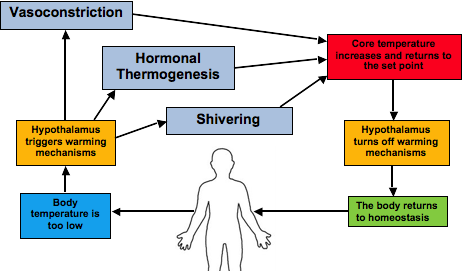
\includegraphics[width=0.3\textwidth]{Figures/figure11.png}
      \caption{Thermoregulation in Response to Cold Body Temperature Stimulus}
      \label{fig:figure11} 
    \end{figure}

  \end{enumerate}
\newpage

\item Question 2
  \begin{enumerate}
  % ANSWER TO 2.1
  \item 

  The ordinary differential equation (ODE) governing the temperature \( T(t) \) is:

  \[
  \frac{dT(t)}{dt} = \frac{Q_f(t) - UA(T(t) - T_a)}{\rho V c_p}
  \]

  For this problem, the furnace is off, so \( Q_f(t) = 0 \). Substituting this into the equation:

  \[
  \frac{dT(t)}{dt} = \frac{-UA(T(t) - T_a)}{\rho V c_p}
  \]

  At steady state, the temperature \( T(t) \) no longer changes with time, so:

  \[
  \frac{dT(t)}{dt} = 0
  \]

  Substitute this condition into the ODE:

  \[
  0 = \frac{-UA(T(t) - T_a)}{\rho V c_p}
  \]

  Solve:

  \[
  T(t) - T_a = 0
  \]

  Thus:

  \[
  T(t) = T_a
  \]

  % ANSWER TO 2.2
  \item
    Using the derived equation for \( T(t) \), the behaviour of the furnace as defined below, and the given definition of one step of the univariate Euler's method, we can plot Figure \ref{fig:figure22}.

  \[
  Q_f(t) =
  \begin{cases} 
  0 & \text{When } T(t) > 23^\circ \text{C}, \\
  1.5 \times 10^6 & \text{When } T(t) < 17^\circ \text{C}, \\
  \text{unchanged} & \text{For all } 17 \leq T(t) \leq 23^\circ \text{C}.
  \end{cases}
  \]

  \begin{figure}[H]
    \centering
    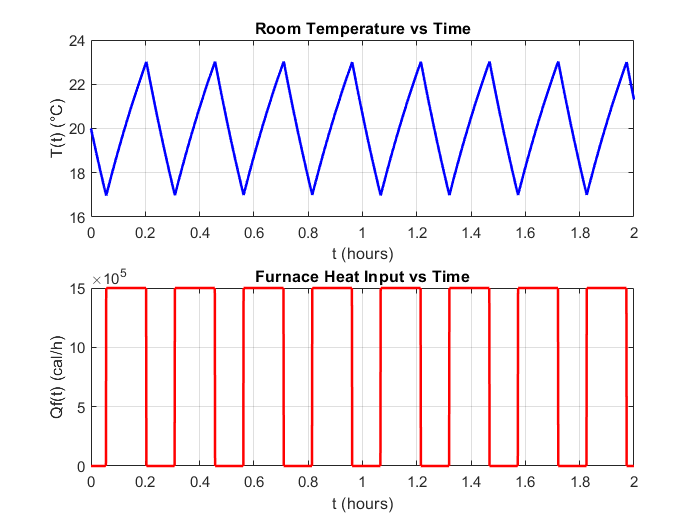
\includegraphics[width=\textwidth]{Figures/figure22.png}
    \caption{Temperature and Furnace Input Over Time}
    \label{fig:figure22} 
  \end{figure}

  % ANSWER TO 2.3
  \item 
  To calculate the number of standard cubic meters of natural gas consumed, we follow the below equation:

  Define $t_{on} \triangleq$  time the furnace was on in hours. The Matlab code says it was 1.182 hours\\
  Define $Q_{f,on} \triangleq$ as the furnace heat input. \\
  Define $\rho_e \triangleq$ as the energy density. \\
  Define $e \triangleq$ as the efficiency. \\

  \[
  \text{Volume of gas consumed} = \frac{t_{on} Q_{f,\text{on}}}{\rho_e e} = \frac{(1.182)(1.5 \times 10^6)}{(9 \times 10^6)(0.9)} = 0.2188888
  \]
  \[
  \approx 0.219 \, \text{standard cubic meters}
  \]

  We also confirm with unit analysis that we get cubic meters.

  \[
  \text{Volume of gas consumed} = \frac{t_{\text{on}} Q_{f,\text{on}}}{\rho_e e} = \frac{\text{hour} \cdot \frac{\text{cal}}{\text{hour}}}{\frac{\text{cal}}{\text{m}^3}} = \text{m}^3
  \]

  % ANSWER TO 2.4
  \item
  With a new oscillating defintion of $T_a$, we get Figure \ref{fig:figure24} below demonstrating the temperature and furnace input over time.

  \begin{figure}[H]
    \centering
    \hspace*{-2.7cm}
    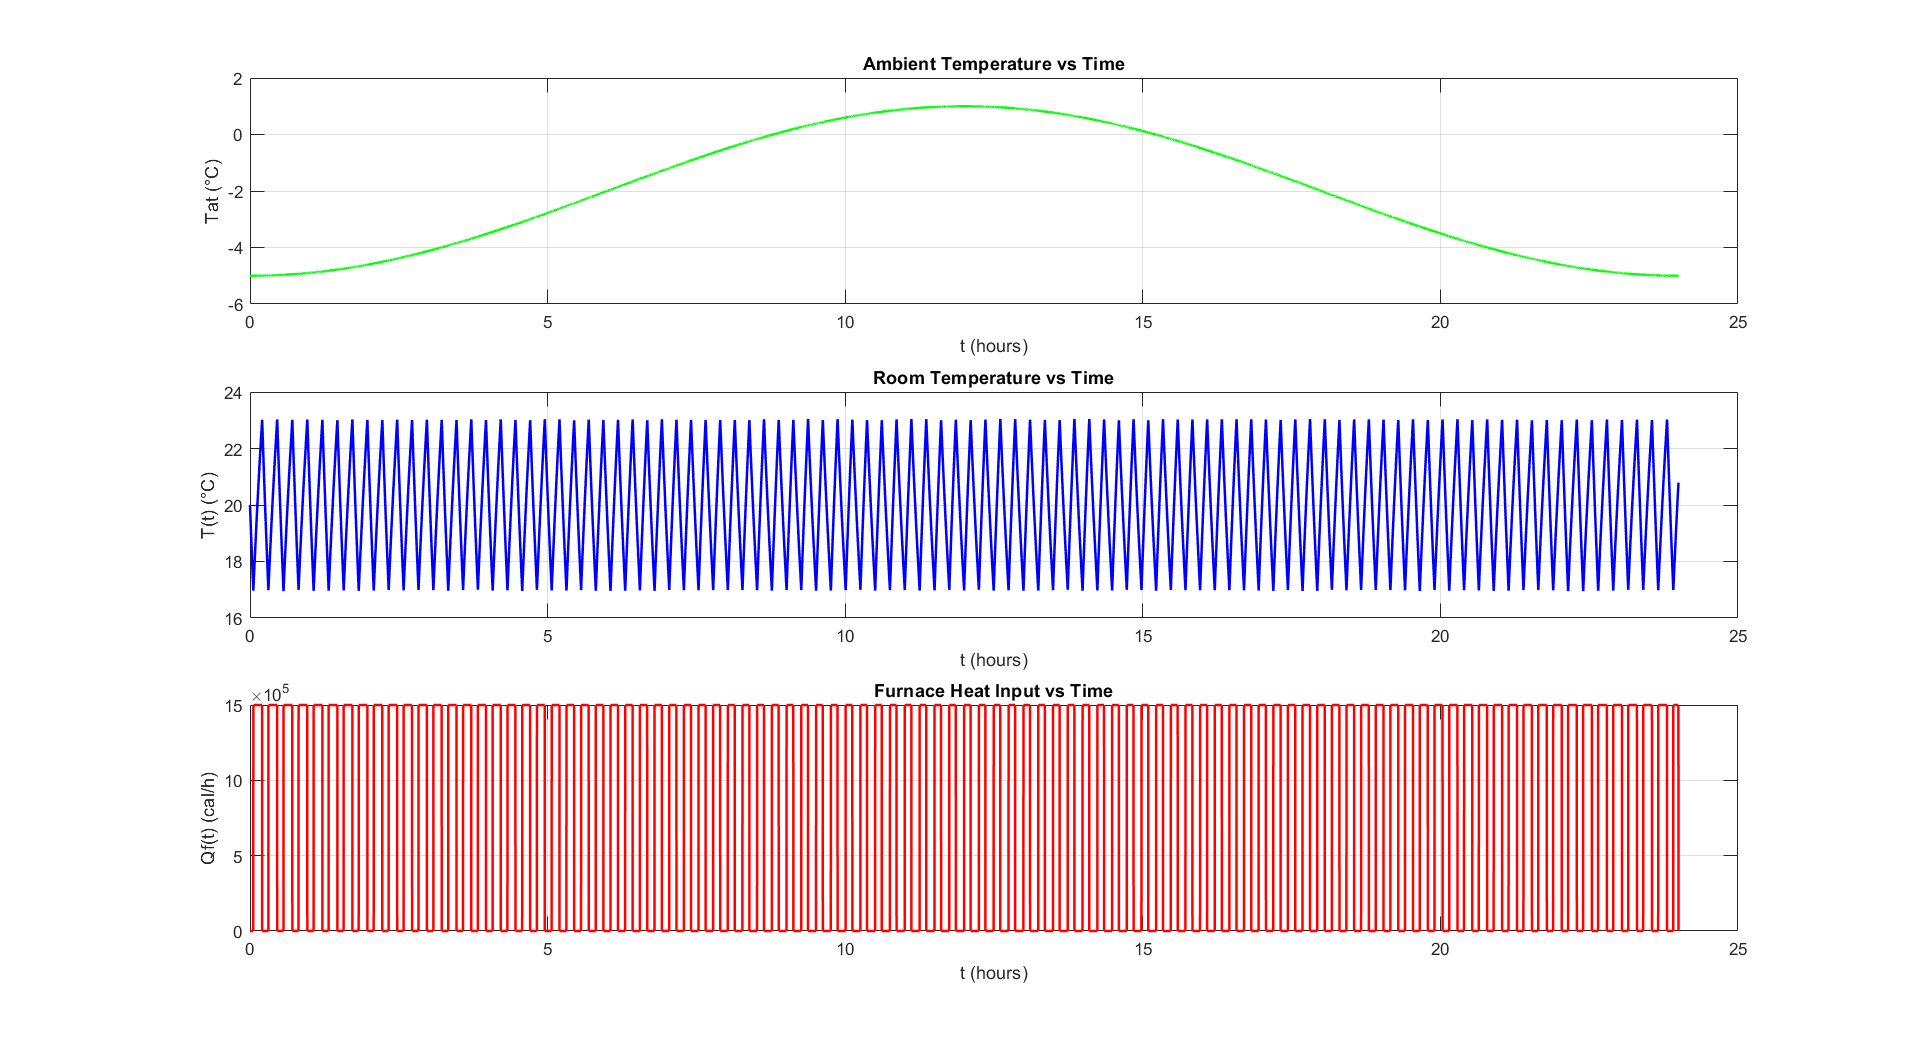
\includegraphics[width=1.3\textwidth]{Figures/figure24real.png}
    \caption{Temperature and Furnace Input Over Time}
    \label{fig:figure24}
\end{figure}

  The simulation results align with the expected behavior of the system. The room temperature \( T(t) \) is maintained within the desired range of \( 17^\circ \text{C} \) to \( 23^\circ \text{C} \) as the furnace responds to changes in the ambient temperature \( T_a(t) \). When \( T_a(t) \) is lower, the furnace operates more frequently to offset increased heat loss, while at higher \( T_a(t) \), the furnace operates less often due to reduced heat loss. By summing the energy added to the room via the furnace over the time it is on over the 24-hour period, we find that \( 1.849 \times 10^7 \) calories of energy were added to the room when the temperature fluctuates. Comparing this to the consistent minimum ambient temperature case from Question 2.2, where \( 2.128 \times 10^7 \) calories were added, we observe a decrease of \( 2.784 \times 10^6 \) calories due to the fluctuating ambient temperature. This is expected, as the furnace operates less frequently when the ambient temperature is higher, resulting in less energy being added to the room.



  \end{enumerate}

  \pagebreak

\item Question 3
  \begin{enumerate}
  % ANSWER TO 3.1
  \item 
    We are given the following ODE describing the current going thorugh the system.

    \[
    V_s(t) = Ri(t) + L\frac{di(t)}{dt}
    \]

    During steady state, the current \( i(t) \) is constant, so the derivative of \( i(t) \) with respect to time is zero. Substituting this into the ODE:

    \[
    V_s(t) = Ri(t) + L(0)
    \]

    Rearranging, we get the following equation for $i(t)$:

    \[
    i(t) = \frac{V_s(t)}{R}
    \]

    This is useful when designing a cirtcuit with a target current i(t) because you can control the voltage source to achieve the desired current while the resistance will always be a constant property of the circuit's hardware. 

  % ANSWER TO 3.2
  \item 
    The results of the Matlab code was plotted below in Figure \ref{fig:figure32}. You can see that it plateaus to a value of 0.1. We know $V_s(t)$ was defined as a constant $5 V$ and R as $50 \Omega$. We know the steady state is $\frac{V_s(t)}{R}$ which in this case would give us $0.1 A$, so we can see that the plot shows our steady state expression holds.

    \begin{figure}[H]
      \centering
      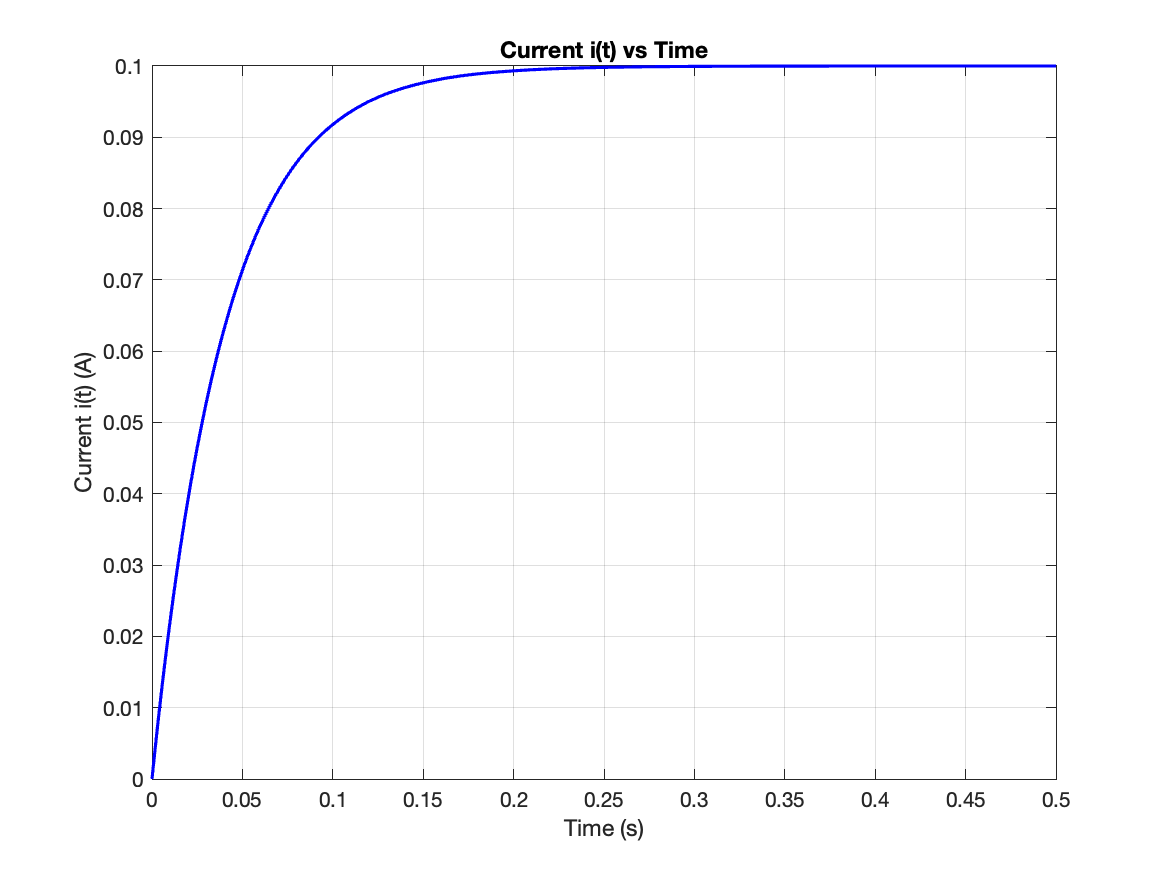
\includegraphics[width=\textwidth]{Figures/figure32.png}
      \caption{Current Over Time}
      \label{fig:figure32}
    \end{figure}

  % ANSWER TO 3.3
  \item 
    
    \[
    V_s(t) = Ri(t) + L\frac{di(t)}{dt}
    \]
  
    Based on the ODE above, inductance $L$ should have no effect on the steady state current $i(t)$ because the derivative of $i(t)$ with respect to time is zero, and inductance is a coeffecient on the derivative. This means that the inductance $L$ term in the ODE will not affect the current $i(t)$ when the system reaches steady state, and the current $i(t)$ will be determined solely by the voltage source $V_s(t)$ and the resistance $R$ in the circuit. This can be seen below in Figure \ref{fig:figure33}, where changing R causes the steady state current $i(t)$ to change, while changing L has no effect on the steady state current $i(t)$.

    \begin{figure}[H]
      \centering
      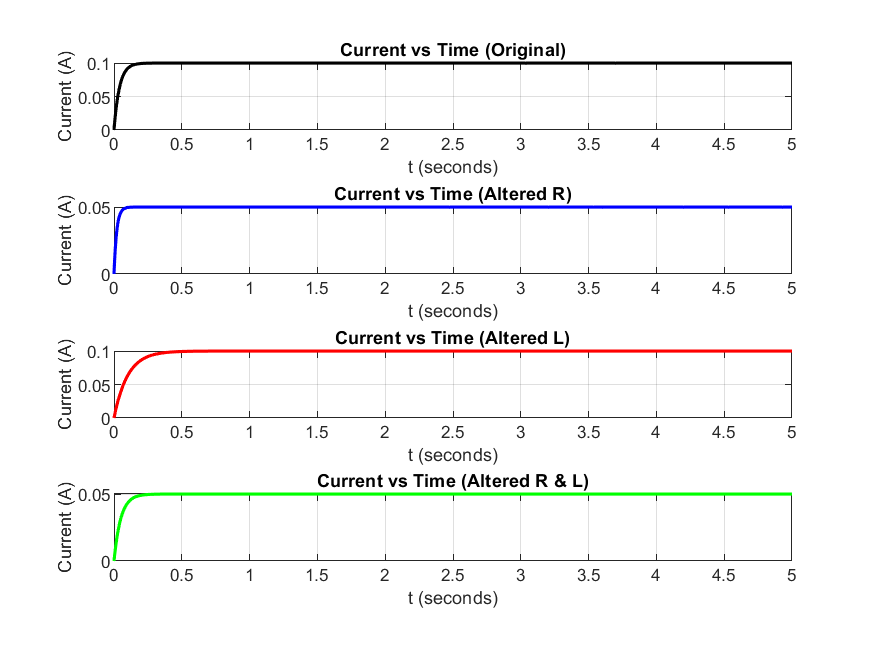
\includegraphics[width=\textwidth]{Figures/figure33.png}
      \caption{Current Over Time}
      \label{fig:figure33}
    \end{figure}
  
    % ANSWER TO 3.4
    \item
      Figure \ref{fig:figure34a} and \ref{fig:figure34b} below demonstrates the LTI nature of the system. An LTI system is defined as a system that is both Linear and Time Invariant. A linear system is one that follows the condition that if $x(t) = \alpha x_1(t) + \beta x_2(t), \text{ then } y(t) = \alpha y_1(t) + \beta y_2(t)$. That is, the output of a system is a linear combination of the inputs. We can observe in \ref{fig:figure34a} that the combination of the inputs $V_s1 = 5V$ and $V_s2 = 10V$ results in the outputs $i_1(t)$ and $i_2(t)$, which is equal to $i_3(t)$.$i_3(t)$ is the resultant output from the combination input of $V_s3 = V_s1 + V_s2 = 15V$. This is exhibits the linear property. We can also observe the system is time-invariant by looking at the equation --- the equation has no coeffecients that change over time. We can also see in \ref{fig:figure34b} that when taking the input and adding time delay, it is equivalent to taking the original output and time shifting that. This proves the equation is time-invariant.

    \begin{figure}[H]
      \centering
      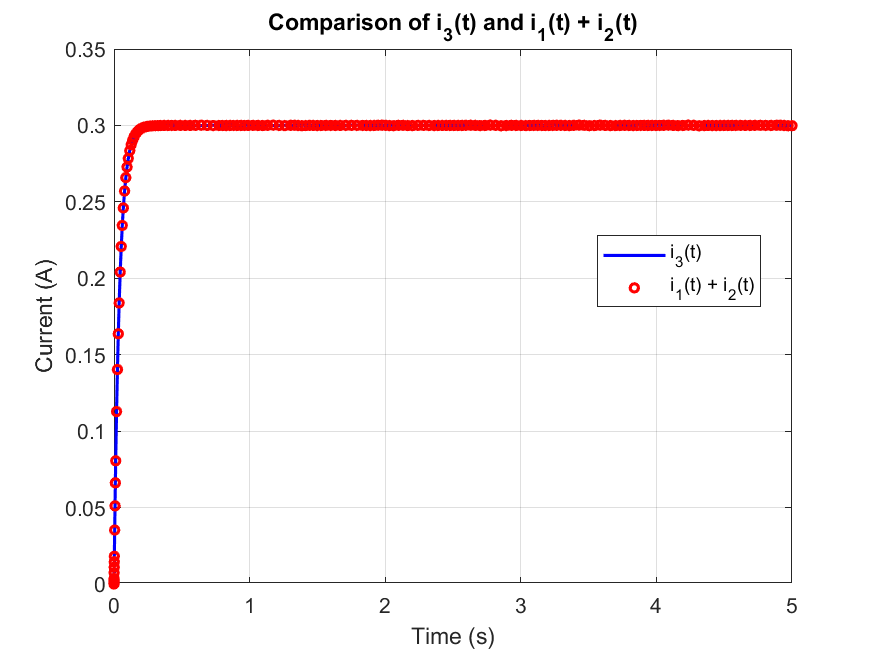
\includegraphics[width=\textwidth]{Figures/figure34.png}
      \caption{Comparing Linear Combination of Inputs to an Equivalent Output Over Time}
      \label{fig:figure34a}
    \end{figure}

    \begin{figure}[H]
      \centering
      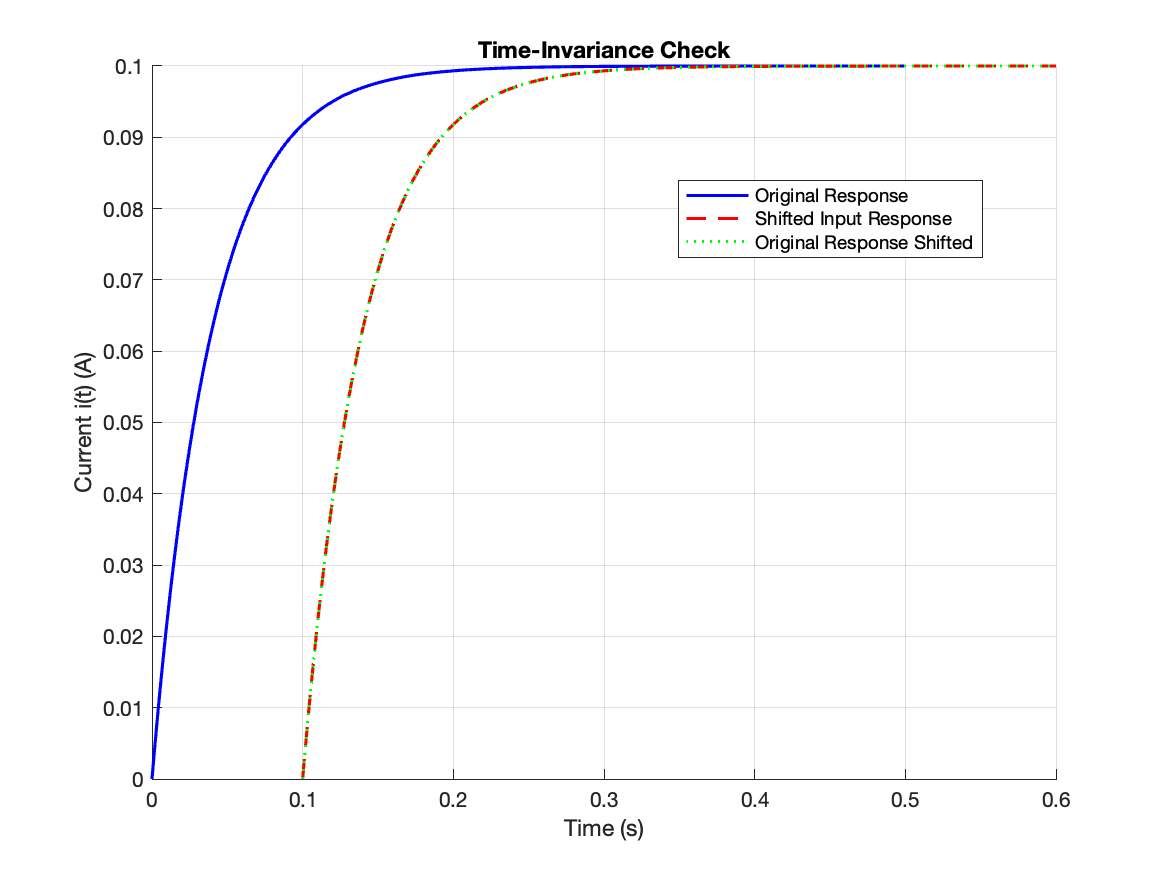
\includegraphics[width=\textwidth]{Figures/figure35.png}
      \caption{Comparing a Time-Shifted Input with the Time-Shifted Output of the Original Signal}
      \label{fig:figure34b}
    \end{figure}

  \end{enumerate}
\newpage

\item Question 4
  \begin{enumerate}
  \item The SIRV model was simulated for 40 years without any vaccination. The initial conditions were set as follows: 
  \begin{itemize}
      \item Susceptible population: \( S(0) = 14,750 \)
      \item Infected population: \( I(0) = 250 \)
      \item Recovered population: \( R(0) = 85,000 \)
      \item Vaccinated population: \( V(0) = 0 \)
  \end{itemize}

  From the plot in Figure \ref{fig:figure41}, we observe that:
  \begin{itemize}
      \item The susceptible population \( S(t) \) initially declines sharply due to the rapid spread of the infection but stabilizes around 5,900 after repeated infection cycles.
      \item The infected population \( I(t) \) experiences periodic outbreaks initially but these periodic outbreaks seem to decrease significantly after the 10 year mark, approaching near 0 levels. It is interesting that the infected near the end of the 40 years is still around 60.
      \item The recovered population \( R(t) \) increases over time and stabilizes around 94,000 as most of the population gains immunity or recovers from the infection. It can be seen that the recovered population is almost the inverse of the susceptible population since as people get infected and recover, they are removed from susceptible.
      \item The vaccinated population \( V(t) \) remains 0 since there was no vaccine in this scenario.
  \end{itemize}

  \begin{figure}[H]
    \centering
    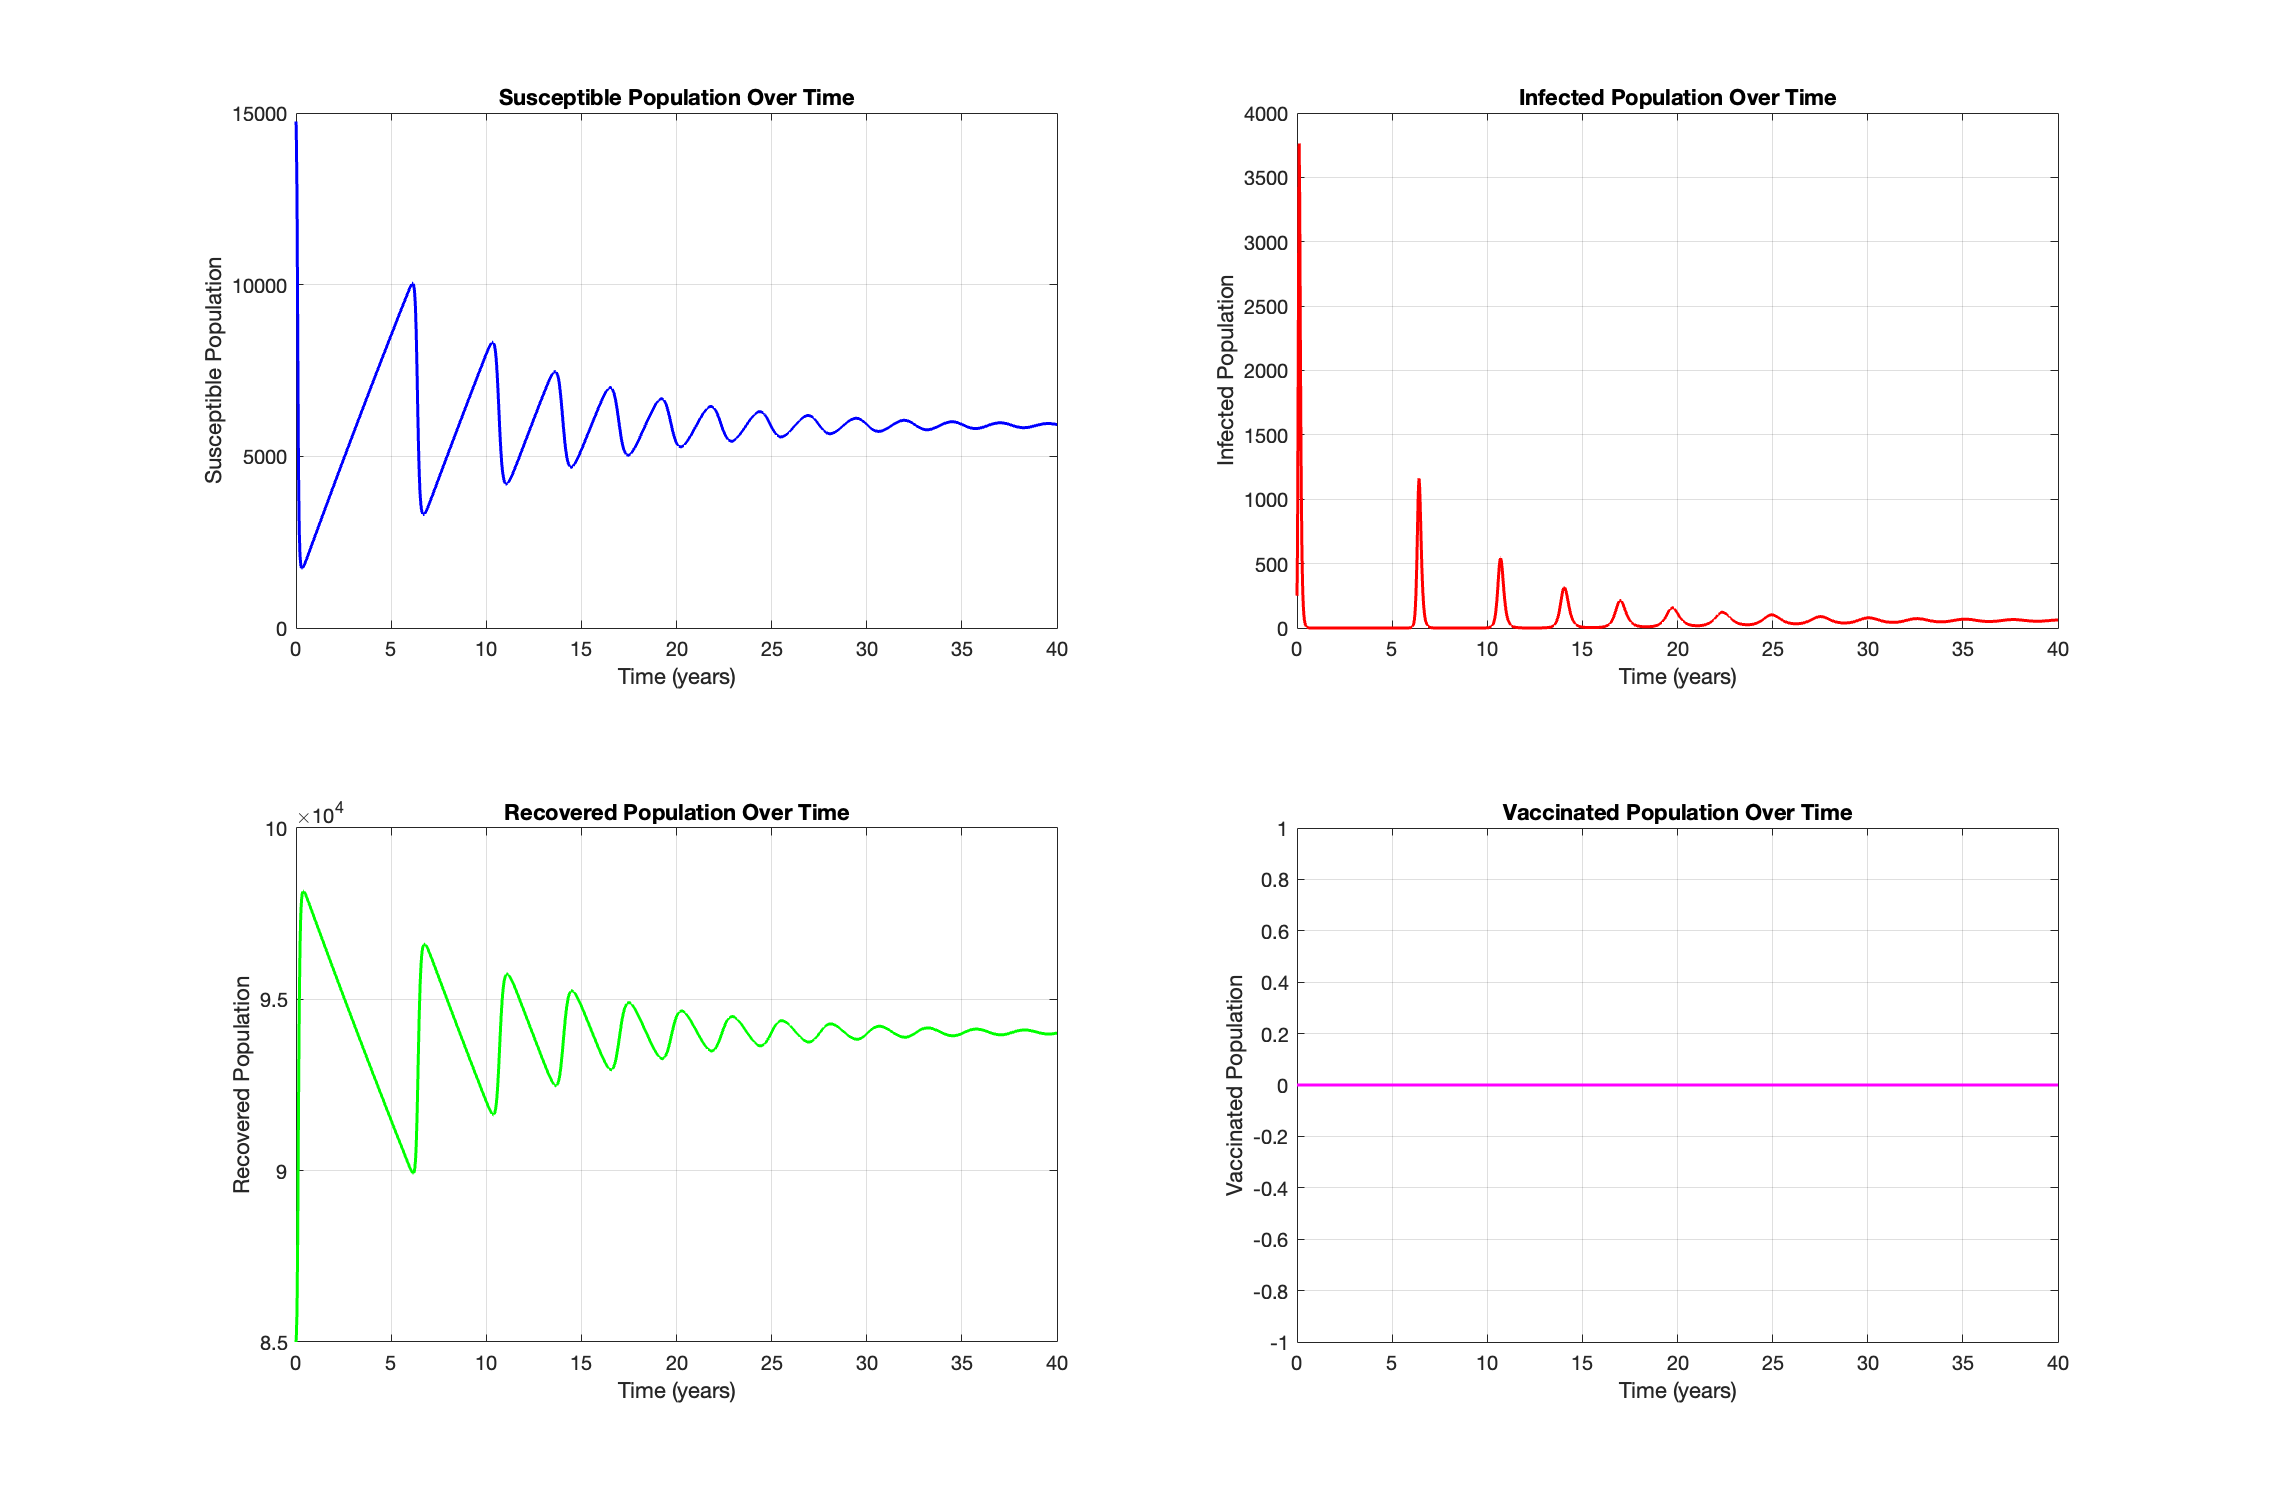
\includegraphics[width=\textwidth]{Figures/figure41.png}
    \caption{Plotting the susceptable, infected, recovered, and vaccinated population for scenario 4.1.}
    \label{fig:figure41}
  \end{figure}

  \item In this scenario, a vaccine is introduced at year 5 with effectiveness \( \epsilon = 0.95 \) and a vaccination rate of \( p = 0.75 \). The initial conditions remain the same as in 4.1.

  From the plot in Figure \ref{fig:figure42}, we observe:
  \begin{itemize}
      \item Before year 5, the dynamics are similar to the results in 4.1, with periodic outbreaks and a declining susceptible population.
      \item After year 5, vaccination is rolled out, leading to a decrease in the infection cycles. The outbreaks are less frequent and severe. The infected population is around 0 at the end of the 40 years here.
  \end{itemize}
  
  The introduction of vaccination after year 5 effectively reduces the effect of the periodic outbreaks, leading to better control of the disease.

  \begin{figure}[H]
    \centering
    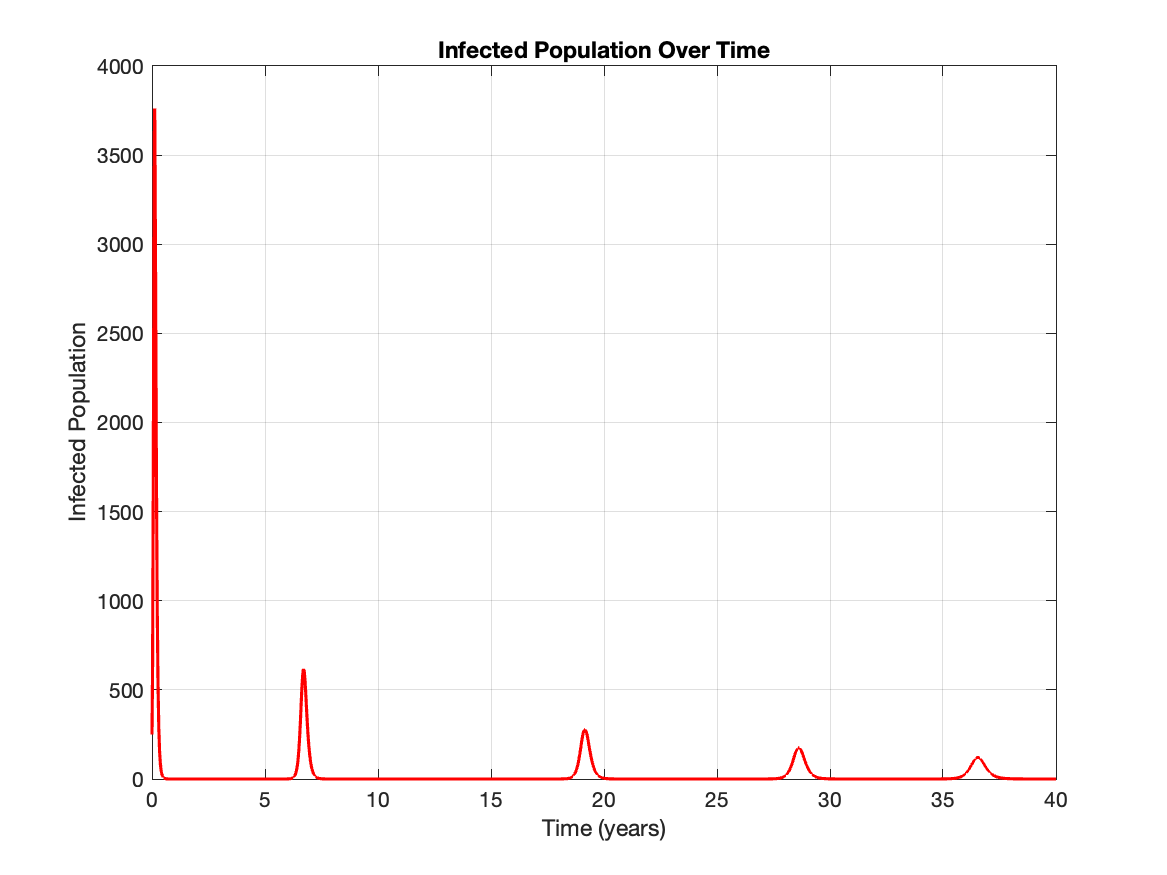
\includegraphics[width=\textwidth]{Figures/figure42.png}
    \caption{Plotting infected population for scenario 4.2.}
    \label{fig:figure42}
  \end{figure}

  \item In this scenario, the critical vaccination rate \( p_c \) was calculated to satisfy the condition \( \epsilon p_c > 1 - \frac{1}{R_0} \) so that we could guarantee the disease be eradicated.

  From the plot in Figure \ref{fig:figure43}, we observe:
  \begin{itemize}
      \item The infected population \( I(t) \) declines rapidly and effectively approaches zero within the first 10 years.
      \item The vaccination rollout significantly reduces the number of outbreak cycles to just 1 close to after year 5 which prevents further outbreaks. The number of infected individuals stabilizes to near 0.
  \end{itemize}
  
  This scenario demonstrates that achieving a critical vaccination rate leads to the eradication of the disease within a reasonable timeframe, as shown by the absence of future outbreaks.

  \begin{figure}[H]
    \centering
    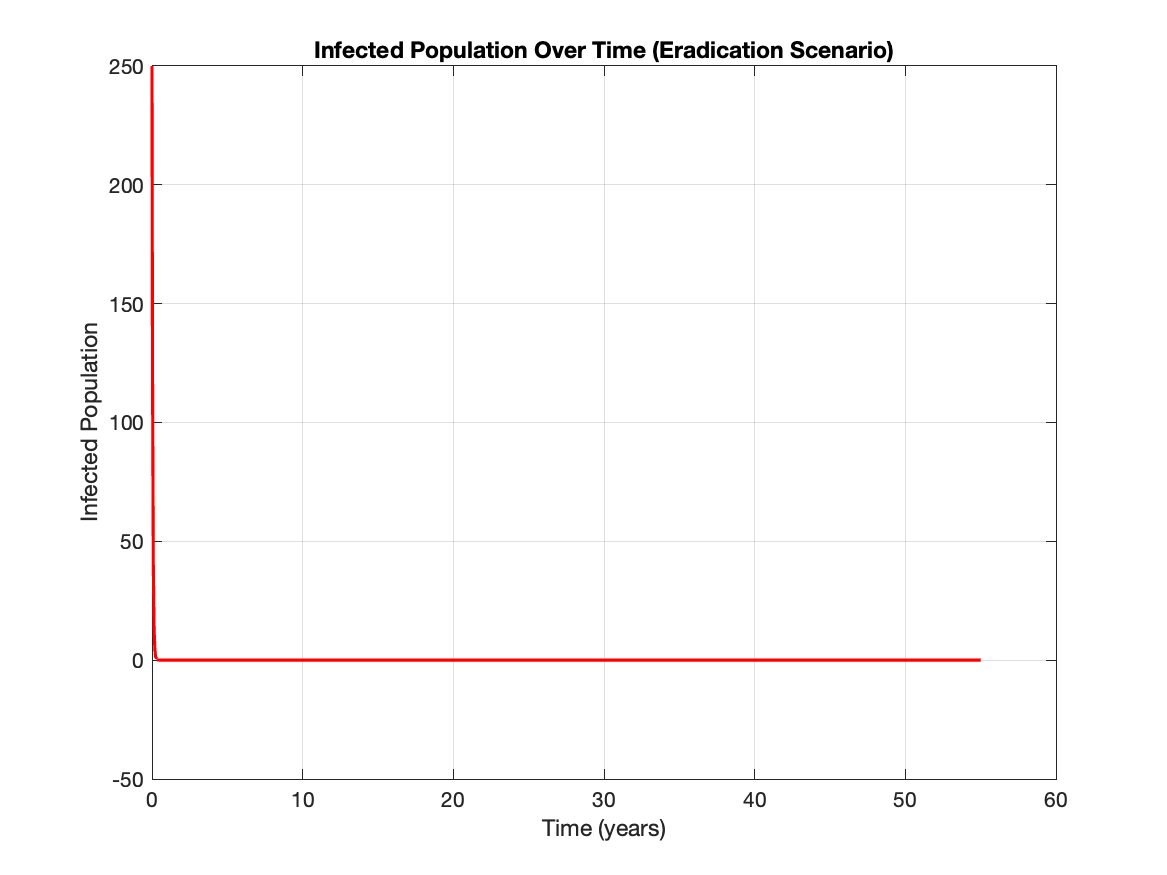
\includegraphics[width=\textwidth]{Figures/figure43.png}
    \caption{Plotting infected population for scenario 4.3.}
    \label{fig:figure43}
  \end{figure}
  
  \end{enumerate}
\newpage

\item Question 5
  \begin{enumerate}
  \item We are given the second-order differential equation:
  \[
  2 \frac{d^2 x(t)}{dt^2} + 3 \frac{dx(t)}{dt} - 2 x(t) = t e^{-2t}
  \]

  Applying the Laplace transform to the differential equation:
  \[
  2 \big[ s^2 X(s) - s x(0) - \dot{x}(0) \big] + 3 \big[ s X(s) - x(0) \big] - 2 X(s) = \mathcal{L} \big( t e^{-2t} \big)
  \]
  Given initial conditions \( x(0) = 0 \) and \( \dot{x}(0) = -2 \), this simplifies to:
  \[
  2 \big[ s^2 X(s) + 2 \big] + 3 s X(s) - 2 X(s) = \frac{1}{(s + 2)^2}
  \]
  \[
  2 s^2 X(s) + 4 + 3 s X(s) - 2 X(s) = \frac{1}{(s + 2)^2}
  \]
  \[
  X(s) \big( 2 s^2 + 3 s - 2 \big) + 4 = \frac{1}{(s + 2)^2}
  \]
  \[
  X(s) \big[(s + 2) (2s - 1) \big] + 4 = \frac{1}{(s + 2)^2}
  \]
  \[
  X(s) = \frac{1 - 4 (s + 2)^2}{(s + 2)^3 (2s - 1)}
  \]

  \item \subsection*{Step 1: Partial Fraction Expansion}
  We decompose \( X(s) \) as:
  \[
  X(s) = \frac{A}{s + 2} + \frac{B}{(s + 2)^2} + \frac{C}{(s + 2)^3} + \frac{D}{2s - 1}
  \]
  Multiply through by the common denominator \( (s + 2)^3 (2s - 1) \):
  \[
  1 - 4 (s + 2)^2 = (s + 2)^2 (2s - 1) A + (s + 2) (2s - 1) B + (2s - 1) C + (s + 2)^3 D
  \]

  \subsection*{Step 2: Determine the Coefficients}
  \subsubsection*{1. Substitute \( s = -2 \) to find \( C \)}
  \[
  1 - 4(s + 2)^2 = (s + 2)^2 (2s - 1) A + (s + 2) (2s - 1) B + (2s - 1) C + (s + 2)^3 D
  \]
  When \( s = -2 \):
  \[
  s + 2 = 0 \quad \Rightarrow \quad (s + 2)^2 = 0 \quad \text{and} \quad (s + 2)^3 = 0
  \]
  This simplifies the equation to:
  \[
  (2s - 1) C = 1 - 4(0)
  \]
  At \( s = -2 \), \( 2(-2) - 1 = -5 \), so:
  \[
  -5 C = 1 \quad \Rightarrow \quad C = -\frac{1}{5}
  \]

  \subsubsection*{2. Substitute \( s = \frac{1}{2} \) to find \( D \)}
  When \( s = \frac{1}{2} \):
  \[
  2s - 1 = 0 \quad \Rightarrow \quad (2s - 1) = 0
  \]
  \[
  (s + 2)^3 D = 1 - 4 \bigg( \frac{5}{2} \bigg)^2
  \]
  \[
  s + 2 = \frac{1}{2} + 2 = \frac{5}{2}
  \]
  \[
  1 - 4 \bigg( \frac{5}{2} \bigg)^2 = 1 - 4 \cdot \frac{25}{4} = 1 - 25 = -24
  \]
  \[
  \bigg( \frac{5}{2} \bigg)^3 D = -24 \quad \Rightarrow \quad \frac{125}{8} D = -24
  \]
  \[
  D = -\frac{24 \cdot 8}{125} = -\frac{192}{125}
  \]

  \subsubsection*{3. Substitute \( s = 0 \) to find \( A \)}
  When \( s = 0 \):
  \[
  1 - 4 (s + 2)^2 = (s + 2)^2 (2s - 1) A + (s + 2) (2s - 1) B + (2s - 1) C + (s + 2)^3 D
  \]
  \[
  s + 2 = 2 \quad \text{and} \quad 2s - 1 = -1
  \]
  \[
  1 - 4(2)^2 = (2)^2 (-1) A + (2)(-1) B + (-1) C + (2)^3 D
  \]
  \[
  1 - 16 = 4(-1) A - 2B - C + 8D
  \]
  \[
  -15 = -4A - 2B - C + 8D
  \]
  Substitute \( C = -\frac{1}{5} \) and \( D = -\frac{192}{125} \):
  \[
  -15 = -4A - 2B - \bigg( -\frac{1}{5} \bigg) + 8 \bigg( -\frac{192}{125} \bigg)
  \]
  \[
  -15 = -4A - 2B - \frac{307}{125}
  \]
  \[
  -1568 = -500A - 250B
  \]
  \[
  \frac{1568}{250} = 2A + B
  \]
  Simplify:
  \[
  \frac{784}{125} = 2A + B
  \]

  \subsubsection*{4. Substitute \( s = 1 \) to find the second equation for \( A \) and \( B \)}

  When \( s = 1 \):
  \[
  1 - 4(s + 2)^2 = (s + 2)^2(2s - 1)A + (s + 2)(2s - 1)B + (2s - 1)C + (s + 2)^3D
  \]
  Substitute into the equation:
  \[
  1 - 4(3)^2 = (3)^2(1)A + (3)(1)B + (1)C + (3)^3D
  \]
  \[
  -35 = 9A + 3B + C + 27D
  \]
  Substitute \( C = -\frac{1}{5} \) and \( D = -\frac{192}{125} \):
  \[
  -35 = 9A + 3B - \frac{1}{5} + 27 \bigg( -\frac{192}{125} \bigg)
  \]
  \[
  -35 = 9A + 3B - \frac{5210}{125}
  \]
  \[
  -\frac{167}{75} = 3A + B
  \]

  \subsubsection*{5. Solve the system of equations}
  We have:
  \[
  2A + B = \frac{784}{125}
  \]
  \[
  3A + B = -\frac{167}{75}
  \]

  Subtract the first equation from the second:
  \[
  (3A + B) - (2A + B) = -\frac{167}{75} - \frac{784}{125}
  \]
  \[
  A = -\frac{2}{25}
  \]

  Substitute \( A = -\frac{2}{25} \) into \( 2A + B = \frac{784}{125} \):
  \[
  2 \bigg( -\frac{2}{25} \bigg) + B = \frac{784}{125}
  \]
  \[
  B = \frac{784}{125} + \frac{4}{25} = -\frac{2}{25}
  \]
  These are the final values for the partial fraction:
  \[
  A = \frac{96}{125}, B = -\frac{2}{25}, C = -\frac{1}{5}, D = -\frac{192}{125}
  \]

  \subsection*{Step 3: Inverse Laplace Transform}
  We now take the inverse Laplace transform of each term:
  \[
  X(s) = \frac{96}{125} \cdot \frac{1}{s + 2} - \frac{2}{25} \cdot \frac{1}{(s + 2)^2} - \frac{1}{5} \cdot \frac{1}{(s + 2)^3} - \frac{192}{125} \cdot \frac{1}{2s - 1}
  \]

  Using the Laplace table, performed the inverse Laplace and got the time domain solution:
  \[
  x(t) = \frac{96}{125} e^{-2t} - \frac{2}{25} t e^{-2t} - \frac{1}{10} t^2 e^{-2t} - \frac{192}{250} e^{t/2}
  \]

  \item As you can see in Figure \ref{fig:figure51} below, plotting both the numerical solution (using ode45) and the analytical solution (the time domain solution we solved in 5.2), they are equivalent over the time shown.
  
  \begin{figure}[H]
    \centering
    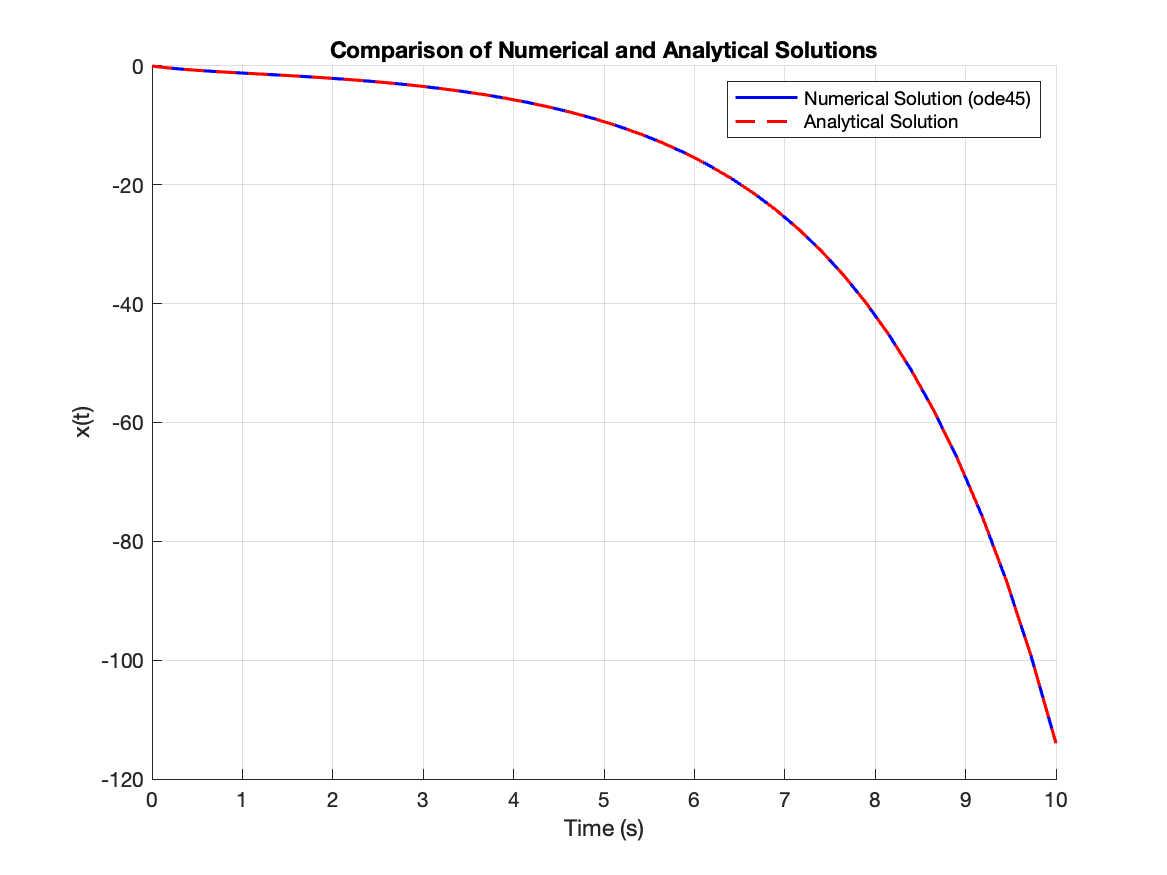
\includegraphics[width=\textwidth]{Figures/figure51.png}
    \caption{Plotting the Numerical vs Analytical Solution}
    \label{fig:figure51}
  \end{figure}

  \end{enumerate}
\newpage

\end{enumerate}

% \pagebreak

% \begin{thebibliography}{9}
%   \bibitem{matlab_ode45}
%   MATLAB Documentation: \texttt{ode45}. Available at: 
%   \url{https://www.mathworks.com/help/matlab/ref/ode45.html}.
% \end{thebibliography}

\end{document}
